\chapter{Literature Review} \label{chap:litreview}

	Robust and fast methods for computing chemical equilibrium in complex systems are widely used in materials and chemical industries. While industrial applications essentially require calculation tools capable of discriminating between stable and unstable phases and converging to nontrivial solutions, numerical equilibrium calculations have historically focussed on representing dominant chemical reactions using the Law of Mass Action. It was only during and after World War {II} that numerical approaches amenable to computer programming were developed. Since then, there has been significant growth in the number of methods and softwares for solving the equilibrium thermodynamics problem.
	
\section{Numerical Methods for Thermodynamic Equilibrium}
	Up until the 1940s, chemical equilibria computations were based on two different methods. The first relied heavily on the assumption that only a few molecular species would be present in the final equilibrium and the law of mass action could be applied to these systems and the resulting system of non-linear equations was solvable using the relatively unsophisticated techniques of the time. The second method relied on a tedious trial-and-error approach with the user's intuition playing a significant role \cite{vanZeggeren11}. It was only during the Second World War that, fuelled by the development of rockets, research towards developing computational methods for chemical equilibrium gained momentum. This research was mainly driven by the fact that an accurate knowledge of chemical equilibrium of the propellants was a requirement for the design of rockets. However, all the methods developed at the time were based on the law of mass action and the procedure was not scalable to very large systems where it would be difficult to account for all the possible reactions.

	The first major breakthrough in computerising chemical equilibrium calculations was made after the Second World war. In 1946, Brinkley came up with a generalised scheme to approach equilibrium computation by giving an analytical criterion for the number of independent components in a multi-component system \cite{vanZeggeren11}. However, the most significant breakthrough in the calculation of thermodynamic equilibria was made at the RAND Corporation by White, Johnson and Dantzig  \cite{White:58}. Since then a few other methods have been proposed but none has found as much success as the method proposed by White et al. In fact, even the method proposed by White et al. has only undergone a few minor changes and more recent algorithm developments have focussed on other complimentary routines, such as initialisation, describes later. This section reviews the major methods that have been proposed to compute thermodynamic equilibria.

	\subsection{Equilibrium constants}
	The earliest computational method for finding thermodynamic equilibrium relied on the equilibrium constants of individual reactions and were primarily applied to gas phase equilibria. The equilibrium constant, $K$, is defined as follows:
	\begin{equation}\label{eq:eqbconst}
		K = \frac{\prod^{N_p} x_{i,p}^{\nu_i}}{\prod^{N_r} x_{i,r}^{\nu_i}},
	\end{equation}
	where $x_{i,p}$ and $x_{i,r}$ denote the mole fractions of species $i$ in product and reactants respectively, $\nu_i$ denotes the stoichiometric coefficient of $i$, and, $N_p$ and $N_r$ denote the number of product and reactants, respectively.

	While equation~\eqref{eq:eqbconst} is easily applicable to single reactions, calculating the concentration of species in multiple simultaneous reactions each with a unique equilibrium constant is quite laborious. The first computational procedure for the calculation of the composition at chemical equilibrium of systems of many constituents was proposed by Brinkley \cite{Brinkley:1947aa} and is known as \emph{Brinkley's method}. Subsequently, a number of modifications were made to this method resulting in a number of other variant methods, such as the \emph{Brinkley-Krieger-White method} \cite{Krieger:1948aa}, the \emph{NASA method} \cite{Zeleznik:1968aa}, etc. The Brinkley-Krieger-White method, also known as the \emph{Brinkley-Newton-Raphson} method, is perhaps the most popular and, as is evident from the name, used the Newton-Raphson method to solve the system of non-linear equations \cite{vanZeggeren11}. The NASA method \cite{Zeleznik:1968aa} shares the same fundamentals as the Brinkley's method.

	Although Brinkley's method serves well for small systems suitable for hand calculations, it relies heavily on user intuition and prior knowledge of the reactions taking place. Furthermore, it neglects the effects of non-ideality and its derivatives due to mathematical difficulties \cite{Zeleznik:1968aa}. Eventually, owing to generalities and numerical superiorities of the Gibbs Energy Minimisation (GEM) method, the Brinkley method fell out of favour among the scientific community.

	\subsection{Computing thermodynamic equilibria}
	The numerical technique of minimising the Gibbs energy of the system was originally proposed by White, Johnson and Dantzig \cite{White:58} and is based on the method of steepest descent of second order and was therefore referred to as the \emph{Second Order Steepest Descent Method}. This methodology, now commonly described as \emph{Gibbs energy minimisation}, has also been called as the \emph{RAND method} owing to the employer of the developers of the method.

	Gibbs energy minimisation is based on identifying a unique combination of species and phases that yield a minimum in the integral Gibbs of a closed isothermal isobaric system from amongst the many possible candidates. The selection of candidates is based on the first and second laws of thermodynamic and is subject to the conditions of thermochemical equilibrium -- satisfaction of the Gibbs phase rule, conservation of mass. Numerically, this amounts to systematically adjusting the Lagrangian multipliers -- some which represent the chemical potential of the system components -- to change the estimated amount of each species, making the Gibbs energy of the system progressively more negative.

	While the initial popularity of the GEM method was fuelled by its generality,  reduced dependence on user intuition and convenience of programmability \cite{Zeleznik:1968aa}, several other advantages have become more apparent as time progressed. Boynton advanced the method to include stoichiometric phases coexisting with solution phases \cite{Boynton:1960aa} and Eriksson \cite{Eriksson:1975aa} demonstrated the use of the method for non-ideal solutions and showed that when dealing with multiple solution phases, the numerics does not get significantly complicated. In fact, the number of simultaneous linear equations to be solved is equal to the number of system components and the number of phases estimated to be stable at equilibrium \cite{vanZeggeren11,Boynton:1960aa,Eriksson:1975aa,Eriksson73}.

	Over a period of time, a number of other techniques have been proposed for the thermochemical equilibrium problem. Most of them, however, have relied on the original GEM method \cite{White:58} as the fundamental approach with minor modifications to adapt to the nature of specific problem at hand. These modifications include accounting for charged species \cite{ERIKSSON1979375}, accounting for non-traditional effects such as surface tension \cite{KOUKKARI200618}, magnetic ordering \cite{Eriksson90} and Donnan effect \cite{PAJARRE200658}. Some of the more significant variations, such as the \emph{First Order Steepest Descent Method} proposed by Storey and van Zeggeren \cite{Storey:1964aa}, demonstrated poorer performance and lacked the ability to distinguish between local minima and maxima \cite{Storey:1964aa,vanZeggeren11}. Another variation relies on removing the mass balance constraint resulting in an unconstrained optimisation problem. This method, proposed by Lantagne et al. and based on a penalty function using the Broyden-Fletcher-Goldfarb-Shanno (BFGS), technique simultaneously minimises two objective functions - Gibbs energy of the system and the residual of the mass constraint vector \cite{LANTAGNE1988589,Nocedal06}. The method must also satisfy the linear inequality constraints related to mole numbers being non-negative. While the approach offers the advantage of solving fewer linear equations, the dual optimisation method is less numerically stable compared to single optimisation methods \cite{Nocedal06}.

	An impediment in numerically solving thermodynamic equilibria is the requirement of an initial estimate for the optimisation. Eriksson and Thompson \cite{Eriksson89} proposed a method called \emph{Levelling}, which is capable of closely estimating the dominant species and their quantities in the phase assemblage. The process requires a relatively small number of iterations and the number of iterations to reach convergence does not rapidly increase with the number of species in the system. These characteristics of levelling are well suited to large systems, such as nuclear materials. Another problem that arises when using GEM method is the negative mole fraction arising due to the evaluation of logarithmic term while computing the chemical potentials. White et al. proposed using a numerical dampening technique to avoid erroneous results. Finally, ensuring that the Gibbs energy of the system is at global minimum and not at one of the many local equilibria is a significant challenge that must be handled properly to ensure correct results. Despite the challenges, GEM has been shown to be the best available method for computing thermodynamic equilibrium and is the de-facto default solver in almost all the thermodynamic equilibrium codes.

	\subsection{Partitioning of Gibbs energy (PGE)}
	The developer of Gibbs energy minimisation, W.B. White, proposed another numerical technique named \emph{Partitioning of Free Energy}  \cite{White67}, which is substantially different from the GEM method. In this method, the mass equations are differentiated with respect to Lagrange multipliers and though a number of numerical advantages were shown, the method was only applicable to homogeneous systems comprised of ideal gas and could not be used for heterogeneous systems involving pure stoichiometric phases and/or multiple solution phases \cite{White67,vanZeggeren11}. The significant disadvantages of this method compared to GEM led to it being mostly dismissed by the thermodynamic community until Piro \cite{Piro11b} reconsidered a modified form of the method by incorporating principles of the levelling method and employed it in an earlier version  of thermochemistry library {Thermochimica} \cite{Piro13}.

	Piro's approach \cite{Piro13} constrains  Gibbs' phase rule  while iterating to satisfy the mass balance constraint. The method constrains the chemical potential of all species and phases in terms of the chemical potentials of the system components, thus formally relating the mass balance equations to the chemical potentials of the system components. The objective of the method is to partition the Gibbs energy of the system among the elements to minimise the residuals of the mass balances. Thus, in this method, the solver attempts to find the roots of the mass balance residual vector while the Gibbs criteria is inherently verified and need not be verified at every iteration thus simplifying the numerical approach. This approach can then be used for heterogeneous systems, which may include stoichiometric phases, ideal solution phases and even non-ideal solution phases.

	Numerically, GEM is an optimisation procedure while PGE solves for the roots of a simultaneous system of linear equation \cite{vanZeggeren11}. As a result, the chemical potential terms for the solution phase are included in the GEM method but absent from the functional vectors in PGE. Additionally, the approaches differ in the computation of a new set of mole numbers, which must be positive. Computation of non-negative logarithmic terms can result in non-real numbers in GEM causing numerical difficulties and necessitating the use of numerical dampening which in turn reduces the rate of convergence. However, in PGE, additional dampening is not required since the mole fractions, being defined as exponentials of real numbers, will always be positive.

	A disadvantage of the PGE method is that it requires moles fractions to be explicitly expressed as functions of chemical potentials of the species. As shown before, chemical potentials of the species can be uniquely expressed as a functions of mole fraction but not the other way around. Thus for non-ideal species, the PGE method fails in the absence of explicit functions of mole fractions in terms of chemical potentials. Despite all its numerical advantages, the PGE method proved to be less robust than the GEM approach and was eventually replaced by GEM in Thermochimica. Though promising, the method has only been used in a limited number of other applications, a couple of them being by Riel et al. \cite{Riel:2022aa} and by Kruskopf \cite{Kruskopf:2018aa}.

	\subsection{Other methods}
	Several other numerical methods have been proposed for computing thermodynamic equilibria but none has received success like GEM. The most notable of these is the approach by Srinivas and Rangaiah which uses  the Random Tunnelling Algorithm (RTA) based on the concept of Terminal Repeller and Unconstrained Subenergy Tunnelling (TRUST) algorithm \cite{Srinivas06}. The TRUST algorithm is akin to the steepest descent method but differs in that the minimisation is performed in two stages - a local minimisation followed by global minimisation through tunnelling \cite{Nocedal06}.  However, the method is limited by the system size and shows satisfactory performance for relatively small systems of up to 10 variable \cite{Nocedal06}.

	Another method that was proposed by the developers of the GEM method is based on linear programming. George B. Dantzig applied the Simplex method to thermodynamic equilibrium problem at constant temperature and pressure \cite{Dantzig:1957aa,Dantzig:1958aa}. In the simplex method, a linear approximation of Gibbs energy of the system is minimised instead of the non-linear system. The linearised model is obtained by representing the logarithmic function in the chemical potential term by the following:
	\begin{equation}
		\beta_i = \alpha_i \ln \alpha_i
	\end{equation}
 which is represented as a piecewise linear approximation as shown in fig.~\ref{fig:simplex}.
 	\begin{figure}[htbp]
		\centering
		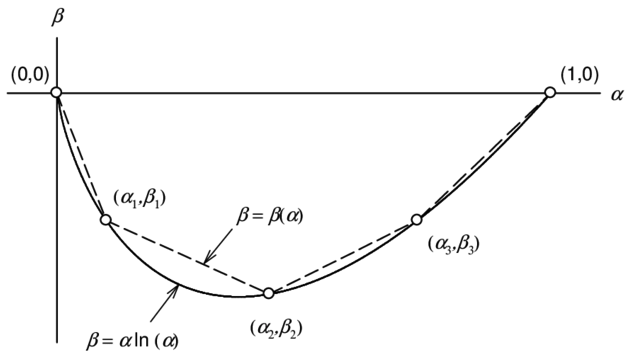
\includegraphics[width=0.75\textwidth]{figures/Simplex}
		\caption[Approximation of the function $\beta$ in simplex method.]{Approximation of the function $\beta$ in Simplex method. Reproduced by Piro \cite{Piro11b} from Dantzig et al. \cite{Dantzig:1957aa}}
		\label{fig:simplex}
	\end{figure}
	Though the Simplex method has been successful in many optimisation problems \cite{Dantzig:2016aa}, the linearisation of $\beta$ generates a relatively large number of additional unknowns and the computational expense becomes quite large. Furthermore, the method is unable to determine the composition of dilute species \cite{vanZeggeren11}. As a result, the simplex method has not received widespread usage in thermodynamic equilibrium calculations.


\subsection{Gibbs energy minimisers (GEM)}
	Over the years, a number of codes have been developed to compute thermodynamic equilibria in complex systems and many of these codes are summarised in table~\ref{tab:gemreview}. The most noticeable of these codes include SOLGAS \cite{Eriksson71} and its successor SOLGASMIX \cite{Eriksson:1975aa}, which are well known for their versatility, computational efficiency and the widespread availability of source code. In fact, SOLGAS has been used as the solver in codes like HSC \cite{HSCSoftware:aa}, ChemSage \cite{Eriksson90} and FACT \cite{Thompson83}. FACT combined the thermodynamic equilibrium solver with a comprehensive thermodynamic database and, by implementing the levelling method, eliminated the need for the user to manually input initial estimates. This made FACT a popular choice in the thermodynamics community. FACT merged with ChemSage to create a new standalone software called FactSage \cite{Bale02}, which is the current version of the SOLGAS family. Another app in the family, called ChemApp \cite{Eriksson:2008aa,Petersen:2007aa}, is a software library that can be called from external codes and has similar capabilities as FactSage.

	Another family of popular thermodynamic equilibria tools is ThermoCalc \cite{ANDERSSON2002273} and is widely used in thermodynamic model development, thermodynamic equilibrium calculations, and  phase diagram construction. It has been developed for complex heterogeneous interaction systems with strongly non-ideal solution phases and can be applied to any thermodynamic system in the fields of chemistry, metallurgy, material science, alloy development, geochemistry, semiconductors etc. depending on the kind of database it is connected to. A unique advantage of ThermoCalc compared to other thermodynamic codes is that it allows explicit conditions on individual phase compositions or configuration whereas most software can handle conditions on the overall composition only. For example, activities and chemical potentials of the components, volumes, enthalpies, entropies etc can also be set as conditions.  OpenCalphad \cite{Sundman:2015aa} is an open-source code led by Bo Sundmann, one of the original developers of ThermoCalc, and it aims to provide facilities for multicomponent equilibrium calculations using the Compound Energy Formalism (CEF) and other models both for interactive calculations and in application software. It has been designed to allow interested scientists to develop thermodynamic models and assess model parameters for thermodynamic databases to describe experimental data as well as theoretical results from DFT calculations to calculate phase equilibria and phase diagrams. Another notable code developed with the goal of enabling uncertainty quantification is PyCalphad developed by Otis et al. \cite{Otis:2017aa}.

	Amongst the many thermodynamic equilibrium codes available in the open literature, one of the common limitations pertains to the relatively small number of standalone calculations that these codes are designed to perform. While suitable for problem specific calculations, where a few failures in convergence would have no significant bearing on the performance, these codes cannot be integrated into multiphysics softwares. In addition, since the mathematical difficulty in achieving convergence increases with the number of phases that can coexist in the system, most of these softwares  limit the maximum number of phases and system components that can be simultaneously considered. While this has no bearing on applications such as combustion, the limited number of phases that can be solved creates a severe impediment for nuclear applications.

	In the nuclear materials community, three code families have garnered particular attention - GEMINI \cite{Cheynet09}, ThermoCalc \cite{ANDERSSON2002273} and FactSage \cite{Bale02}. Due to their established reputation in the nuclear community, these codes have traditionally been applied in development of several thermodynamic treatments for nuclear fuels and materials. In fact these three codes offer a number of advantages over the other codes reviewed here, including the capability of handling a very large number of system components, phases and species, and the ability to use a wide range of sophisticated thermodynamic models.
	
{%\newgeometry{margin=1cm}
%%\begin{landscape}
%\pagestyle{empty}
%		\begin{longtable}{p{0.15\textwidth} p{0.25\textwidth} p{0.1\textwidth} p{0.125\textwidth} p{0.125\textwidth} p{0.125\textwidth} p{0.125\textwidth}}
\renewcommand{\arraystretch}{0.7}
	\begin{longtable}{@{}lclcrcrcrcr@{}}
		\caption{A review of the major thermodynamic equilibrium codes.}\\
		\toprule
		\multicolumn{1}{c}{\multirow{2}{*}{\textbf{Code / Author}}} &\phantom{} & \multicolumn{1}{c}{\multirow{2}{*}{\textbf{Method}}} &\phantom{} & \multicolumn{7}{c}{\textbf{Models}} \\
		\cmidrule{5-11}
		\multicolumn{1}{c}{} & \phantom{} & \multicolumn{1}{c}{} & \phantom{} & \multicolumn{1}{c}{\textbf{Stoich.}} & \phantom{} & \multicolumn{1}{c}{\textbf{Ideal}} & \phantom{} & \multicolumn{1}{c}{\textbf{Non-ideal}} & \phantom{} & \multicolumn{1}{c}{\textbf{Ionic}} \\
		\midrule
		\endfirsthead
		\caption[]{A review of the major thermodynamic equilibrium codes (contd).}\\
		\toprule
		\multicolumn{1}{c}{\multirow{2}{*}{\textbf{Code / Author}}} &\phantom{} & \multicolumn{1}{c}{\multirow{2}{*}{\textbf{Method}}} &\phantom{} & \multicolumn{7}{c}{\textbf{Models}} \\
		\cmidrule{5-11}
		\multicolumn{1}{c}{} & \phantom{} & \multicolumn{1}{c}{} & \phantom{} & \multicolumn{1}{c}{\textbf{Stoich.}} & \phantom{} & \multicolumn{1}{c}{\textbf{Ideal}} & \phantom{} & \multicolumn{1}{c}{\textbf{Non-ideal}} & \phantom{} & \multicolumn{1}{c}{\textbf{Ionic}} \\
		\midrule
		\endhead
		ANGE (SAGE) \cite{Baurens:2014aa} && GEM && Yes && Yes && Yes && Yes \\
		CALMIX \cite{GREINER1988529} && GEM && Yes && Yes && Yes && No \\
		Cantera \cite{Goodwin:aa} && GEM && No && Yes && Yes && No \\
		Castier et al. \cite{CASTIER1989237} && GEM && No && Yes && No && No \\
		CatCalc \cite{Shobu09} &&GEM && Yes && Yes && Yes && No \\
		CEA \cite{Gordon94} && GEM && Yes && Yes && No && No \\
		ChemApp \cite{Eriksson:2008aa} && GEM && Yes && Yes && Yes && Yes\\
		ChemSage \cite{Eriksson90} && GEM && Yes && Yes && Yes && Yes\\
		ChemSheet \cite{Koukkari:2005aa} && GEM && Yes && Yes && Yes && Yes\\
		COEXIST \cite{Ahafat:1992aa} && Levelling && Yes && No && No && No\\
		Dantzig et al. \cite{Dantzig:1958aa}&& Simplex && No && Yes && No && No\\
		Ebel et al. \cite{Ebel:2000aa} && BNR && Yes && Yes && No && No\\
		ESP \cite{Rafal:2003aa} && LMA && No && Yes && No && No\\
		FACT \cite{Thompson83} && GEM && Yes && Yes && Yes && Yes\\
		FactSage \cite{Bale83} && GEM && Yes && Yes && Yes && Yes\\
		GEMINI 1 \cite{Cheynet09} && GEM && Yes && Yes && No && No\\
		GEMINI 2 \cite{Cheynet09} && GEM && Yes && Yes && Yes && Yes\\
		GEM-Selektor \cite{Karpov:aa} && GEM && Yes && Yes && No && Yes\\
		GEMIPM2K \cite{Karpov:aa} && GEM && Yes && Yes && No && Yes\\
		Gibbs \cite{COOL2010393} && C-Hull && {} && Yes && Yes && {}\\
		GLOPEQ \cite{MCDONALD19971} && GEM* && No && Yes && No && No\\
		HALTA \cite{Sillen:1962aa} && LMA && No && Yes && No && No\\
		HALTAFALL \cite{INGRI19671261} && LMA && Yes && Yes && No && No\\
		Han et al. \cite{HAN1998897} && LMA* && No && Yes && No && No\\
		HSC \cite{HSCSoftware:aa} && GEM && Yes && Yes && Yes && Yes\\
		Koukkari et al. \cite{KOUKKARI200618} && Const. GEM && Yes && Yes && Yes && Yes\\
		Kruskopf \cite{Kruskopf:2018aa} && PGE && Yes && Yes && Yes && Yes\\
		Lantagne et al. \cite{LANTAGNE1988589} && {GEM} && No && Yes && Yes && No\\
		Lee et al. \cite{PENGLEE19991183} && {GEM} && No && Yes && Yes && No\\
		Lukas et al. \cite{Lukas77} && {GEM} && Yes && Yes && Yes && No\\
		MAGEMin \cite{Riel:2022aa} && {PGE} &&  && Yes && Yes && \\
		MatCalc \cite{Kozeschnik:2001aa} && {GEM} &&  && Yes && Yes && \\
		MTDATA  \cite{Davies02} && {GEM} && No && Yes && Yes && No\\
		NUTS \cite{Loukusa:2014aa} && {GEM} && Yes && Yes && Yes && Yes\\
		OpenCalphad \cite{Sundman:2015aa} && {GEM} && Yes && Yes && Yes && Yes\\
		PANDAT \cite{Cao09} && {GEM} && Yes && Yes && Yes && Yes\\
		Pereira et al. \cite{PEREIRA20101} && {HEM} && No && Yes && No && No\\
		PyCalphad \cite{Otis:2017aa} && {Lower C-Hull} && Yes && Yes && Yes && No\\
		Rossi et al. \cite{ROSSI20111226} && GEM && Yes && Yes && No && No\\
		Schnedler \cite{SCHNEDLER1984265} && GEM && Yes && Yes && No && No\\
		Smith and Missen \cite{Smith:1988aa} && GEM && No && Yes && No && No\\
		SOLGAS \cite{Eriksson71} && GEM && No && Yes && No && No\\
		SOLGASMIX \cite{Eriksson:1975aa} && GEM && Yes && Yes && Yes && No\\
		SOLGASMIX-PV \cite{Besmann:1977aa} && GEM && Yes && Yes && Yes && No\\
		SOLGASWATER \cite{ERIKSSON1979375} && GEM && Yes && Yes && Yes && Yes\\
		Song et al. \cite{SONG19912513} && GEM* && Yes && Yes && No && No\\
		Srinivas et al. \cite{Srinivas06} && GEM-RTA && No && Yes && No && No\\
		STANJAN / EQUIL \cite{Reynolds86} && PGE && No && Yes && No && No\\
		Storey et al. \cite{Storey:1964aa} && GEM && Yes && Yes && No && No\\
		THERIAK \cite{DECAPITANI19872639} && GEM && No && Yes && Yes && No\\
		ThermoCalc \cite{ANDERSSON2002273} && GEM && Yes && Yes && Yes && Yes\\
		Thermochimica \cite{Piro13} && GEM && Yes && Yes && Yes && Yes\\
		ThermoSolver \cite{Piro11b} && PGE && Yes && Yes && Yes && Yes\\
		VICTORIA \cite{Heams:1992aa} && LMA && Yes && Yes && No && No\\
		White et al. \cite{White:58} && GEM && No && Yes && No && No\\
		NASA \cite{Zeleznik:1968aa} && NASA && No && Yes && No && No\\
		\bottomrule\label{tab:gemreview}
	\end{longtable}
%%\end{landscape}
%\restoregeometry
}
	
	\section{Global Optimisation}
	Calculation of thermodynamic equilibrium is a challenging problem since the objective functions are multivariable and can often be non-convex and highly non-linear. Furthermore, additional complexities arise near the phase boundaries, in the vicinity of critical points, etc. \cite{Wakeham04,TEH2002745}. Over the years, a number of different methods have been proposed to find the global minimum for non-convex problems in the applied mathematics community. These methods can be classified into stochastic and deterministic methods. However, even with a large number of different methods available in the literature, finding a method that can be applied to all types of problems has proven impractical. The success of every method is problem-specific and most of the methods reported in the literature have focussed on either relatively small systems, such as liquid-vapour equilibria, or perform relatively small number of calculations.

	\subsection{Deterministic methods}
	Deterministic optimisation methods exploit the analytical properties of the problem to generate a deterministic sequence of points converging to a global optimum \cite{PARDALOS2000209}. While these methods can provide a guaranteed global optimum, they require certain properties of objective function and constraints such a continuity and convexity. These methods include the \emph{Branch and Bound algorithm}, \emph{Homotopy Continuation Methods}  and \emph{Interval Analysis} \cite{Floudas99}.

	The branch and bound algorithm is a class of adaptive partitioning strategies that iteratively apply partitioning, sampling and subsequent upper and lower bounding procedures to solve global optimisation problems \cite{Floudas99}.  These methods typically rely on some \textit{a priori} knowledge of the form of the objective function to  develop convex terms of the optimisation problem. However, they are often computationally expensive and slow \cite{Wakeham04,Nichita02} because the method recursively splits the search space into smaller subspaces and performs function evaluations within each subspace. The homotopy continuation method provides a smooth transition between an approximate solution (often linear) and the true solutions of a non-linear system of equations by gradually introducing the non-linearities through a scalar homotopy parameter \cite{B.-Riggs:1994aa,JALALI20082333}. As a result, the method is capable of finding all roots of a set of non-linear equations. While the method guarantees global convergence to a single solution, it does not guarantee global convergence to multiple solutions. Moreover, the method has been successfully demonstrated only for simple polynomials \cite{Zhang11}.
For the case of thermodynamic equilibrium calculations, Piro and Simunovic \cite{Piro16} have shown that the branch and bound algorithm has proven to be the most promising of all deterministic methods

	\subsection{Stochastic methods}
	By employing probabilistic elements and using random sequences in the search for the global optimum, stochastic methods  provide a high probabilistic convergence to global minimum with little or no assumption on the characteristics of the optimisation problem \cite{Rangaiah:2010aa}. These methods employ heuristics for exploring (diversification) and exploiting (intensification) the search space, and learning strategies are used to find near-optimal solutions at a rapid speed \cite{Blum:2003aa}. This class of optimisation methods include \emph{Random Search}, \emph{Tabu Search}, \emph{Random Tunnelling Algorithm}, \emph{Particle Swarm Optimisation}, \emph{TRUST}, etc.

	The pure random search algorithm by Brooks \cite{Brooks:1958aa} is based on generating a sequence of uniformly distributed points in the search space, while keeping a track of the best point that was already found. The method offers a probabilistic asymptotic guarantee that a global minimum will be found with probability equal to one when the sample size grows to infinity. Luus and Jaakola have proposed an \emph{Adaptive Random Search} algorithm which uses random points and systematic region reduction for locating the global optimum \cite{Luus:1973aa}.

	The Tabu search algorithm proposed by Glover and Laguna \cite{Glover:1993aa} is aimed at enhancing the searching capability of the solution space economically and effectively by discarding the points in the solution space, which have been previously evaluated and found to be not feasible. The method has been successfully applied to a wide range of optimisation problems but  applications to thermodynamic equilibrium computations have been limited \cite{SRINIVAS2007760,Teh03}. One of the other notable algorithms is the random tunnelling algorithm which is a derivative of the TRUST algorithm. The TRUST algorithm \cite{Barhen97} combines the novel concepts of subenergy tunneling, and non-Lipschitzian terminal repellers. In subenergy tunnelling, non-linear transformation is applied to the objective function resulting in the values of the function that are greater than the value at the current local minimum to be set equal to the current minimum. This flattens the search space and the process gets trapped at the current position because the successive gradients remain within the stopping criterion. At this point, the terminal repeller gets activated to allow an escape from the current solution to a point where the function begins another descent. The random tunnelling algorithm. on the other hand, consists of a combination of a local and global phase. In the global phase, the system is randomly perturbed from the last local minimum and a system of differential equations is solved from the perturbed point to explore new regions of attraction. The local phase employs a fast convergent Quasi-Newton minimisation technique to find an improved point in the new region. Amongst the stochastic global optimisation algorithms, Piro and Simunovic \cite{Piro16} have shown that the particle swarm algorithm has proven to be the most promising of all stochastic methods.

	The diversification and intensification plays a key role in ensuring a compromise between reliability and computational efficiency of stochastic algorithms and while the stochastic algorithms can often locate the global minimum in modest computational times compared to deterministic methods, they do not guarantee global optimality \cite{Zhang11,Blum:2003aa}.

	\subsection{Global optimisation review}
	 A few of the studies on global optimisation in thermodynamic equilibrium calculation have been summarised in table~\ref{tab:globalopt}. While most of the global optimisation methods applied to phase equilibrium have been studied with reference to liquid-liquid or vapour-liquid equilibrium, a few of the remarkable ones can be applied to more general phase equilibrium problems. Chaikunchuensakun et al. \cite{Chaikunchuensakun:2002aa} applied a hybrid algorithm based on non-linear parametric optimisation routines which solves the Kuhn-Tucker conditions by minimising a quadratic sub-problem with linearised equality and inequality constraints. While the method can equilibrium solutions, a global solution cannot be guaranteed \cite{Zhang11}. Another notable study is by Nichita et al. \cite{Nichita02} who tested the tunnelling method for multi-phase equilibrium calculation by direct minimisation of Gibbs energy of the components. Rossi et al. \cite{ROSSI20111226} applied a convex analysis method to chemical and phase equilibrium of closed multi-component reactive system. Though the method is highly efficient and reliable, it is only applicable to convex functions. A duality based approach proposed by Pereira et al. \cite{PEREIRA20101} can guarantee the global optimum but requires a differentiable objective function \cite{Zhang11}.

	 Amongst the stochastic methods, the most notable works are from Teh and Rangaiah \cite{Teh03} who show that the tabu search is more efficient that the genetic algorithm but requires further improvement for 100\% reliability. However, the system size considered by them is relatively small. Srinivas and Rangaiah \cite{Srinivas06} used the random tunnelling algorithm which can evaluate the global minimum for most of the examples tested but suffers from low reliability and is feasible only for small systems.

	 In conclusion, the available literature suggests that both deterministic and stochastic methods face difficulties for highly non-ideal mixtures and are prone to convergence problems. Moreover, many of the studies assume the number of phases that would be stable to be known \textit{a priori} which is not true and limits capability. As a result, several calculations must be performed using different combination of phases to arrive at the true global minimum. The global optimisation problem applied to computational thermodynamics warrants a more effective and rigorous study of both deterministic and stochastic methods applied to a variety of case studies with varying levels of complexity. An effort in this direction was made by Piro and Simunovic \cite{Piro16} and they found the PSO and the Branch and Bound algorithms to be the most promising stochastic and deterministic methods, respectively.

%\newgeometry{margin=1cm}
%\begin{landscape}
%\pagestyle{empty}
\begin{table}[ht!]
	\caption{A review of the global optimisation methods applied to thermodynamic equilibrium calculations.}
	\centering
	\begin{tabular}{@{}p{0.45\textwidth} c l c r@{}}
	\toprule
	\multicolumn{1}{c}{\textbf{Method}} &\phantom{a} & \multicolumn{1}{c}{\textbf{Class}} &\phantom{a} & \multicolumn{1}{c}{\textbf{Problem Formulation}}\\
	\midrule
	Sampling \cite{Sundman15,Otis:2017ab} && Deterministic && Gibbs energy \\
	Branch and Bound \cite{CHEUNG2002169} && Deterministic && Potential energy \\
	Branch and Bound \cite{Piro16} && Deterministic  && Gibbs energy \\
	Convex optimisation \cite{ROSSI20111226}&& Deterministic && Gibbs energy \\
	Differential evolution and tabu search \cite{SRINIVAS2007760} && Stochastic && Gibbs energy \\
	Differential evolution with tabu list \cite{Srinivas:2007aa} && Stochastic && Gibbs energy \\
	Duality based optimisation \cite{PEREIRA20101} && Deterministic && Helmholtz energy \\
	Enhanced simulated annealing \cite{ZHU20003451} && Stochastic && Gibbs energy \\
	Enhanced tabu search \cite{Teh03} && Stochastic && Gibbs energy \\
	Genetic algorithm and simulated annealing \cite{Rangaiah01} && Stochastic && Gibbs energy \\
	Genetic algorithm and differential evolution with tabu list \cite{Bonilla-Petriciolet:2011aa} && Stochastic && Gibbs energy with reaction \\
	Hybrid artificial immune system \cite{Lin:2007aa} && Stochastic && Gibbs energy with reaction \\
	Hybrid genetic algorithm with interior point method \cite{STAUDT2009585} && Stochastic && Gibbs energy \\
	Interval analysis \cite{Scurto:2003aa} && Deterministic && Gibbs energy surface \\
	Nonlinear parametric optimisation \cite{Chaikunchuensakun:2002aa} && Deterministic && Gibbs energy \\
	Particle swarm optimisation \cite{Bonilla09,Piro16,Myint:2021aa} && Stochastic && Gibbs energy \\
	Random tunnelling algorithm \cite{Srinivas06} && Stochastic && Gibbs energy \\
	Simulated annealing \cite{Bonilla-Petriciolet:2009aa} && Stochastic && Gibbs energy \\
	Successive quadratic programming \cite{LUCIA20002557} && Deterministic && Gibbs energy \\
	Tunnelling method \cite{Nichita02,Nichita:2004aa} && Deterministic && Gibbs energy \\
	\bottomrule
	\end{tabular}
	\label{tab:globalopt}
\end{table}
%\end{landscape}
%\restoregeometry

\section{Multiphysics Integration of Computational Thermodynamics}

	Interest in incorporating thermodynamic equilibrium calculations in multiphysics simulations has been relatively recent. Even though the importance of thermodynamic variables in various physical simulations has been long recognised, the limitations on computational resources along with the high cost of equilibrium calculations made thermodynamically informed coupled simulations infeasible for most simulations beyond those aimed at purely demonstrating capability. However, over the last few years, the efforts towards coupling thermochemistry have been ever-increasing. Some of such coupling efforts, primarily the ones focused on nuclear applications are reviewed here. 
	
	Most of the applications of coupling computational thermochemistry have been in nuclear fuel codes with some applications in microstructural evolution using phase field method and even lesser applications in safety analyses. A couple of works that have coupled computational thermodynamics with the commercial software package COMSOL include those of Higgs et al. \cite{Higgs:2007aa} and Welland et al. \cite{Welland09}. Piro integrated the thermochemistry solver {Thermochimica} into the Advanced Multi-Physics {AMP} code developed by Oak Ridge National Laboratory \cite{Piro11b}. This allowed the investigation of an irradiated fuel pellet by using isotopic evolution of irradiated nuclear fuel which was calculated through the software package {ORIGEN}. 
% The integration of {Thermochimica} in {AMP} is shown in figure~\ref{fig:amp} and the capabilities of this simulation framework were demonstrated through a scenario that simulates the behaviour of highly irradiated \ce{UO2} fuel, results of which are shown in figure~\ref{fig:pirojnm}.
%	\begin{figure}[htb]
%		\begin{center}
%		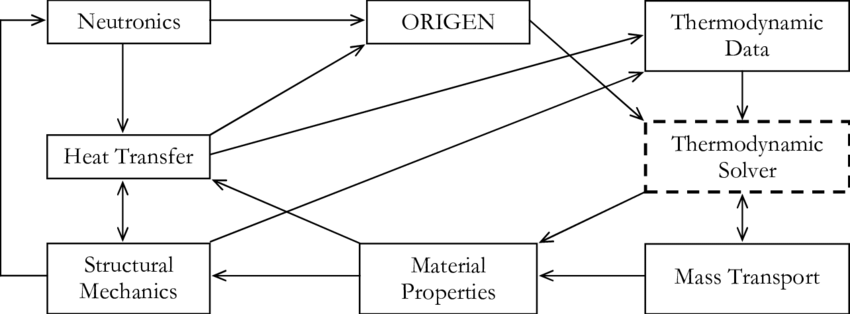
\includegraphics[width=0.75\textwidth]{figures/AMP_TC.png}
%		\caption[A flowchart of the Advanced Multi-Physics (AMP) code illustrating the interaction between the various modules.]{A flowchart of the Advanced Multi-Physics (AMP) code illustrating the interaction between the various modules is shown \cite{Piro11b}.}
%		\label{fig:amp}
%		\end{center}
%	\end{figure}
%	\begin{figure}[htb]
%		\begin{center}
%		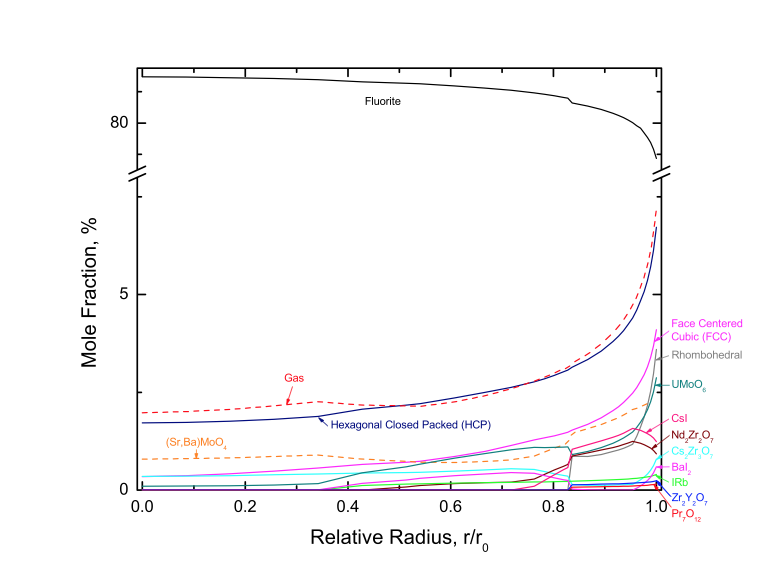
\includegraphics[width=0.85\textwidth]{figures/Piro_JNM}
%		\caption[The predicted distribution of phases across the pellet is shown for an average pellet burnup of 102 GW d t(U)$^{-1}$.]{The predicted distribution of phases across the pellet is shown for an average pellet burnup of 102 GW d t(U)$^{-1}$ \cite{Piro13b}.}
%		\label{fig:pirojnm}
%		\end{center}
%	\end{figure}

	The software integration of Thermochimica with Bison was performed by Simunovic et al. \cite{Simunovic:2020aa}. Use of Thermochimica was demonstrated by modelling oxygen transport in irradiated \ce{UO2} oxide fuel, such as calculation of oxygen to metal ratio in the fluorite phase, oxygen partial pressure, oxygen chemical potential and oxygen transport. Experimental measurements from the open literature were used to validate the implemented models and illustrate functionality of the developed thermodynamics module. The calculations are based on chemical element inventory provided by neutronics, isotopic depletion, transmutation and decay calculations in the \cite{SCALE05} system. To overcome some of the computational cost increase observed by Simunovic et al., Poschmann et al. used a reinitialisation strategy whereby the Thermochimica results were saved at each node at each time step and used to initialise the calculations at the next time step \cite{Poschmann:2019aa}. Poschmann et al. \cite{Poschmann:2021aa} extended the model by  Simunovic et al. to simulate the the \ce{U} and \ce{Zr} interdiffusion in \ce{U-Pu-Zr} metallic fuel. A similar effort by Hirschhorn et al. used Bison as well but with pre-computed thermodynamic values obtained from PyCalphad \cite{Hirschhorn:2021aa}. 

	In France, 3D coupled multiphysics simulations of power ramps in Pressurised Water Reactors (PWR) were performed by Baurens et al. \cite{Baurens:2014aa} and  Konarski et al. \cite{KONARSKI2019104}. The fuel performance code {ALCYONE}, which is part of the computing environment {PLEIADES}, was coupled with the thermodynamics code {ANGE} to provide a description of irradiated fuel thermochemistry with oxygen transport taking into account thermodiffusion. Konarski et al. also performed Pellet Cladding interaction (PCI) failure analyses, by coupling thermochemistry and thermo-mechanics to investigate both chemical and mechanical factors simultaneously. 3D thermochemical-mechanical simulations of PWR power ramps on \ce{Cr}-doped \ce{UO2} with the fuel performance code {ALCYONE} including oxygen transport were performed to study the impact of oxygen redistribution on irradiated fuel thermochemistry and on chemically reactive fission gas release. OpenCalphad has been coupled with ALCYONE for several applications such as those by Michel et al. \cite{Michel:2013aa} and Intro\"{i}ni et al. Intro\"{i}ni et al. proposed multiple coupling strategy to improve the computational performance of the OpenCalphad - ALCYONE coupling and through a set of numerical experiments, demonstrated the performance gain compared to ANGE - ALCYONE coupling. Another code in the PLEIADES environment is Germinal which is specifically aimed at SFR and was coupled to OpenCalphad by Samuelsson et al. \cite{Samuelsson-Karl:2020aa} to model joint oxide cladding.
	
	Use of thermodynamic equilibrium data finds a lot of value in phase field calculations where quantities like Gibbs energy, chemical potentials are all required as inputs. Among the first applications of such coupling were those in the field of metallurgy like those by Grafe et al. \cite{Grafe:2000aa} and Chen et al. \cite{Chen:2005aa} Several other models have been developed with some examples being of those by Zhang et al. \cite{Zhang:2015aa} who directly incorporated Calphad into the phase-field formalism and validated the coupling technique for \ce{Fe-C} and \ce{Ni-Al} alloys and by Schwen et al. \cite{Schwen:2017aa} who used PyCalphad for thermodynamic data in  MOOSE-based phase field application MARMOT. Schwen et al. have also developed a multiphase field model for better integration of thermodynamic phases with multiple sublattices in the phase field model implemented in MOOSE \cite{Schwen:2021aa}. Other similar works include those of B\"{o}ttger et al. \cite{Bottger:2020aa}, Chatterjee and Moelens \cite{Chatterjee:2021aa}, Zuo et al. \cite{Zuo:2021aa} and Coutinho et al. \cite{Coutinho:2022aa}.

	Among other applications, Poschmann et al. \cite{Poschmann:2022aa} coupled Thermochimica to dynamic systems modelling software TRANSFORM for dynamic mass accountancy in liquid-fuelled MSRs and  Fitzpatrick et al. \cite{Fitzpatrick18} coupled Thermochimica with thermal-hydraulics code COBRA-TF and isotopic evolution code ORIGEN to demonstrate fission product transportation by coolant flow in molten salt reactors. Thermochimica has recently been coupled with MELCOR for severe accident modelling in Boiling Water Reactors (BWR) \cite{Breeden:2022aa}.

	Thus, thermodynamic equilibrium calculations have found application in modelling and simulation several physical phenomena. Full integration of a thermodynamic equilibrium code in {MOOSE} would make such coupled calculations easy and allow high fidelity multiphysics simulations allowing much more realistic simulations of various problems. In doing so, however, one must be considerate of the increase in computational cost and should carefully do a cost-benefit analysis before proceeding with such high-fidelity but costly simulations.
